% Chapter 3
\chapter{Data Mining}

\label{Chapter3} 
Pour construire n'importe quel modèle de prédiction, il est nécessaire de choisir une technique d'apprentissage automatique ainsi qu'un Dataset pour entraîner le modèle. Dans ce chapitre nous allons parler des Dataset, comment choisir et évaluer un Dataset. Nous parlerons aussi de l’apprentissage automatique ainsi que de ses deux grandes classes. Cette discipline de traitement de grandes quantité de données et choix de modèles est connue sous le nom de \textit{Data-Mining}.

\section{Data Minig}
\subsection{Définition}
L’exploration de données, connue aussi sous l’expression de fouille de données, forage de données, prospection de données, a pour objet l’extraction d’un savoir ou d’une connaissance à partir de grandes quantités de données, par des méthodes automatiques ou semi-automatiques. Le processus le plus connu du Data-Mining est le KDD (knowledge discovery in database)[\cite{14}], appelé en français extraction de connaissances à partir de données ou processus de découverte de connaissances.

\subsection{Processus KDD}
\label{KDD}
Le processus KDD est composé de trois étapes :\\
\begin{itemize}
\item[1-]\textbf{Préparation des données} : Elle comprend la collecte, l'intégration, la transformation, le nettoyage et la réduction des données. Dans notre cas la Collecte d'information est faite en capturant le trafic réseau à l'aide du \textit{port-mirroring} des équipements réseau.\\
\item[2-]\textbf{Recherche des modèles} : Consiste à appliquer l'analyse des données et les algorithmes de découverte qui produisent une énumération de modèles sur les données.\\
\item[3-]\textbf{Évaluation des modèles} : Consiste à estimer l'erreur et la précision sur les modèles extraits.Un modèle est considéré comme une connaissance s'il dépasse un certain pourcentage de précision.
\end{itemize}

\subsection{Dataset}
Pour concevoir notre modèle d'apprentissage nous avons besoin d'une grande quantité de données qui représentent plusieurs flux, malins et bénins, capturés dans un réseau SDN réel. Le choix du bon Dataset contenant ce type de données est crucial pour construire notre modèle de prédiction. Dans ce qui suit quelques propriétés à prendre en considération lors du choix d'un Dataset [\cite{15}].\\
\begin{itemize}
\item[•]\textbf{Year of Creation}: Étant donné que le trafic réseau est soumis à de nouveaux scénarios d’attaques, l’âge d’un ensemble de données de détection d’intrusion joue un rôle important. Cette propriété décrit l’année à laquelle le trafic a été capturé.\\
\item[•]\textbf{Normal User Behavior}: Cette propriété indique la disponibilité du comportement normal de l’utilisateur dans un ensemble de données et prend les valeurs \textbf{Oui} ou \textbf{Non}. La valeur \textbf{Oui} indique qu’il y a un comportement normal dans l’ensemble de données. En général, la qualité d’un IDS est principalement déterminée par son taux de détection des attaques et son taux de fausses alarmes. Par conséquent, la présence d’un comportement normal est indispensable pour évaluer un IDS.\\
\item[•]\textbf{Attack Traffic}: Un Dataset pour IDS devrait contenir divers scénarios d’attaque. Cette propriété indique la présence de trafic réseau malicieux dans le Dataset.\\
\item[•]\textbf{Kind of Traffic}: La propriété Type de trafic décrit trois origines possibles du trafic réseau : réel, émulé ou synthétique. Réel signifie que le trafic réseau réel a été capturé dans un environnement réseau en production. Émulé signifie que le trafic réseau réel a été capturé dans un banc d’essai ou un environnement réseau émulé. Synthétique signifie que le trafic réseau a été créé synthétiquement (par exemple, par un générateur de trafic) et non capturé par un dispositif réseau réel.\\
\item[•]\textbf{Balanced}: Pour la phase d'apprentissage les données doivent être équilibrés et respecter  leurs étiquettes de classe. Cette propriété indique si le Dataset est équilibré. Un Dataset déséquilibré devrait être équilibré selon des méthodes appropriées, avant de passer à l'algorithme d'apprentissage.\\
\item[•]\textbf{Labeled}: Un Dataset étiqueté est nécessaire pour entraîner et tester les modèles d’apprentissage supervisés et non-supervisés. Cette propriété indique si le Dataset est étiqueté ou non. 
\end{itemize}

\begin{table}[h]
\begin{center}
\begin{tabular}{   m{4cm} | m{10cm}  }
\textbf{Dataset} & \textbf{Attaques}\\
\hline
\rowcolor[rgb]{0.85,0.85,0.85}
CICDoS [\cite{16}]  & Attaques DoS sur la couche d'application (ddossim, Goldeneye, hulk, RUDY, Slowhttptest,Slowloris).\\
\hline
CICIDS 2017 [\cite{17}] & Botnet, DoS, DDoS, infiltration, SSH brute force, Injection SQL.\\
\hline
\rowcolor[rgb]{0.85,0.85,0.85}
CIDDS-001 [\cite{18}] & DoS, port scans, SSH brute force.\\
\hline
DDoS 2016 [\cite{19}] & DDoS(HTTP Flood, ICMP Flood, UDP Flood).\\
\hline 
\rowcolor[rgb]{0.85,0.85,0.85}
CICIDS 2018 [\cite{20}] & DoS, FTP and SSH brute force, Botnet, Infiltaration, DDoS.\\
\hline
CICDDoS 2019 [\cite{21}] & Attaques DDoS Reflectives.\\
\hline
\end{tabular}
\caption{Quelques Datasets disponibles pour les système de détection d'intrusions}
\end{center}
\label{table:Datasets}
\end{table}


\newpage
\section{Apprentissage automatique}
L’apprentissage automatique est un concept de développement, d’analyse et d’implémentation qui permet à une machine d’apprendre d’une manière automatique la résolution de problèmes qui s’avéraient complexes à traiter en utilisant les algorithmes classiques.\\

\noindent L’apprentissage automatique est utilisé pour résoudre plusieurs types de problèmes complexes dont la classification et la régression. Le problème de classification est de classifier des données ou des instances en plusieurs classes selon les caractéristiques de ces derniers. Par exemple, apprendre à reconnaître si un flux est bénin ou malin est un problème de classification binaire ; détecter le type d’une attaque parmi plusieurs types d’attaques possibles est un problème de classification multi-classes. Les problèmes de régressions sont des problèmes d’approximation des valeurs continues d’une certaine fonction. Par exemple, apprendre à prédire la température pour un jour donné connaissant les diverses conditions atmosphériques.\\

\noindent Les algorithmes d’apprentissage automatique sont classés en deux grandes classes. Cette classification est directement liée à l’inclusion ou pas d’étiquettes dans l’ensemble de données.

\subsection{Apprentissage supervisé}
L’apprentissage supervisé est un système qui fournit à la fois les données en entrée et les données attendues en sortie. Les données en entrée et en sortie sont étiquetées en vue de leur classification, afin d'établir une base d'apprentissage pour le traitement ultérieur des données. Les systèmes d'apprentissage automatique supervisé alimentent les algorithmes d'apprentissage avec des quantités connues qui étayeront les futures décisions. Ils sont associés pour la plupart à une intelligence artificielle basée sur la récupération, mais ils peuvent aussi reposer sur un modèle d'apprentissage génératif.\\

\noindent Les données utilisées pour l'apprentissage supervisé sont une série d'exemples comprenant des paires composées de sujets en entrée et de sorties attendues. Les modèles d'apprentissage supervisé présentent certains avantages sur les modèles non supervisés, mais ils ont aussi des limites. Par exemple, ils sont plus susceptibles de prendre des décisions auxquelles les humains peuvent s'identifier parce qu'elles reposent sur des données fournies par les humains. Mais dans le cas d'une méthode basée sur la récupération, les systèmes d'apprentissage supervisé ont des difficultés à traiter les nouvelles informations. Si un système qui connaît deux catégories de flux, le flux d’une attaque SYN-Flooding et le flux bénin par exemple, reçoit un flux d’une attaque UDP-Flooding, il devra le placer dans l'une ou l'autre de ces deux catégories, ce qui sera incorrect. Alors que si le système était génératif, il ne saurait pas forcément reconnaître le type d’attaque UDP-Flooding, mais il serait capable de l'identifier comme appartenant à une autre catégorie. \\

\noindent Parmi les algorithmes d’apprentissage supervisé nous trouvons les machines à vecteur de support (SVM),  AdaBoost (adaptative boosting), k plus proches voisins (k-NN) et les réseaux de neurones convergeant vers un état final précis.

\subsection{Apprentissage non supervisé}
L’apprentissage non supervisé consiste à apprendre à un algorithme d'intelligence artificielle (IA) des informations qui ne sont ni classées, ni étiquetées, et à permettre à cet algorithme de réagir à ces informations sans supervision.\\

\noindent Dans ce mode d'apprentissage, le système d'IA peut regrouper des informations non triées en fonction de leurs similitudes et de leurs différences, même si aucune catégorie n'est indiquée. Les systèmes d'IA capables d'utiliser l'apprentissage non supervisé sont souvent associés à des modèles d'apprentissage génératifs, mais ils peuvent aussi fonctionner avec une approche basée sur la récupération (souvent associée à l'apprentissage supervisé).\\

\noindent Les algorithmes d'apprentissage non supervisé peuvent exécuter des tâches de traitement plus complexes que les systèmes d'apprentissage supervisé, mais ils peuvent aussi être plus imprévisibles. Même si un système d'IA d'apprentissage non supervisé parvient tout seul, par exemple, à faire le tri entre des flux bénins et des flux malins, il peut aussi ajouter des catégories inattendues et non désirées pour y classer des flux inhabituels, créant la confusion au lieu de mettre de l'ordre.
Parmi les algorithmes d’apprentissage non supervisé nous citons K-means clustering (K-moyenne), Dimensionality Reduction (Réduction de la dimensionnalité), Distribution models (Modèles de distribution) et Hierarchical clustering (Classification hiérarchique).\\

\newpage
\paragraph{{\large 3.2.2.1 Clustering}\\\\}
Il s'agit essentiellement d'un type de méthode d'apprentissage non supervisé. Clustering est la tâche de diviser la population ou les points de données en un certain nombre de groupes de sorte que les points de données des mêmes groupes soient plus similaires aux autres points de données du même groupe et différents des points de données des autres groupes. Il s'agit essentiellement d'une collection d'objets sur la base de la similitude et de la dissemblance entre eux.\\

\noindent Le clustering est très important car il détermine le groupement intrinsèque des données non marquées. Il n'y a aucun critère pour un bon clustering. Cela dépend de l'utilisateur. Quels sont les critères qu'il peut utiliser pour satisfaire ses besoins? Par exemple, nous pourrions être intéressés à trouver des représentants pour des groupes homogènes (réduction des données), à trouver des groupements utiles et appropriés (“useful” data classes) ou à trouver des objets de données inhabituels (outlier détection). L'algorithme du clustering doit faire quelques hypothèses qui constituent la similitude des points et chaque hypothèse fait des clusters différents et également valides. 

\paragraph{{\large 3.2.2.2 Méthodes de clustering}\\\\}
Parmi les méthodes de Clustering, nous citons:\\
\begin{itemize}
\item[-]Méthodes basées sur la densité: ces méthodes considèrent les clusters comme la région dense ayant une certaine similitude et différence des autres régions denses de l'espace. Ces méthodes ont une bonne précision et la capacité de fusionner deux clusters. Exemples : DBSCAN, OPTICS …etc.\\
\item[-]Méthodes basées sur la hiérarchie : les clusters formés dans cette méthode forment une structure de type arbre basé sur la hiérarchie. Les nouveaux clusters sont formés en utilisant ceux précédemment formés.\\
\item[-]Méthodes de partitionnement : ces méthodes partitionnent les objets en k clusters et chaque partition forme un cluster. Cette méthode est utilisée pour optimiser une fonction de similarité de critère objectif comme lorsque la distance est un paramètre majeur. Exemple : K-means, CLARANS …etc.
\end{itemize}

\paragraph{{\large 3.2.2.3 K-Means}\\\\}
K-means est un algorithme non supervisé de clustering non hiérarchique. Il permet d’analyser un jeu de données caractérisées par un ensemble de descripteurs, afin de regrouper les données similaires en groupes (ou clusters). La similarité entre deux données peut être inférée grâce à la “distance” séparant leurs descripteurs ; ainsi deux données très similaires sont deux données dont les descripteurs sont très proches. Cette définition permet de formuler le problème de partitionnement des données comme la recherche de K “données prototypes”, autour desquelles peuvent être regroupées les autres données. Ces données prototypes sont appelées centroïdes ; en pratique l’algorithme associe chaque donnée à son centroïde le plus proche, afin de créer des clusters. D’autre part, les moyennes des descripteurs des données d’un cluster, définissent la position de leur centroïde dans l’espace des descripteurs : ceci est à l’origine du nom de cet algorithme (K-means ou K-moyennes en Français). Après avoir initialisé ses centroïdes en prenant des données au hasard dans le jeu de données, K-means alterne plusieurs fois ces deux étapes pour optimiser les centroïdes et leurs groupes:\\
\begin{itemize}
\item[1-]Regrouper chaque objet autour du centroïde le plus proche.
\item[2-]Replacer chaque centroïde selon la moyenne des descripteurs de son groupe.\\
\end{itemize}

Après quelques itérations, l’algorithme trouve un découpage stable du jeu de données : on dit que l’algorithme a convergé. Comme tout algorithme, K-means présente des avantages et des inconvénients : il est simple, rapide et facile à comprendre ; cependant il ne permet pas de trouver des groupes ayant des formes complexes.

\begin{figure}[h]
\centering
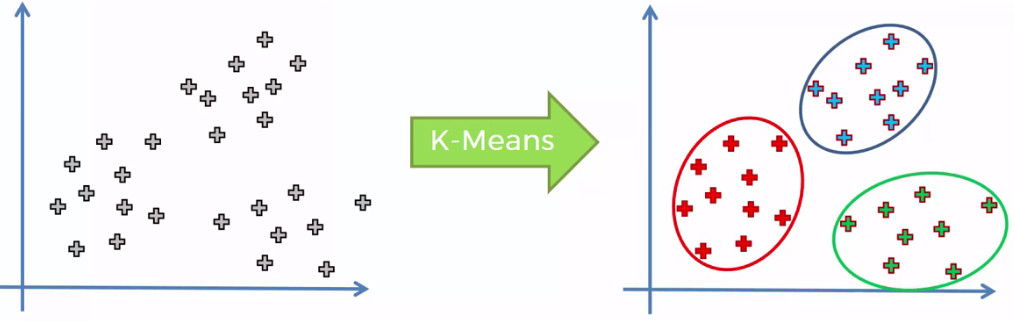
\includegraphics[width=0.8\textwidth]{Figures/K-means}
\decoRule
\caption{K-Means}
\label{fig:K-means}
\end{figure}

\subsection{Conclusion}
Dans ce chapitre nous avons discuté sur le Data-Minig, en commençant par définir ce qu'est cette discipline, pour passer par la suite au dataset en exposant les majeures propriétés à considérer lors du choix d'un dataset. L'apprentissage automatique était la dernière section de ce chapitre, où nous avons présenté les différentes méthodes et algorithmes d'apprentissage existants. 
